% Bagian Tugas Pendahuluan
\section*{Tugas Pendahuluan}
\begin{enumerate}
  \item Jelaskan bagaimana cara kontrol 7-segment anoda dan katoda?
  \begin{enumerate}[label=\alph*.]
    \item 7-segment Anoda \\
    Pada display tujuh segmen dengan anoda umum, semua anoda dari segmen-segmen terhubung bersama, sementara setiap segmen memiliki koneksi katoda yang terpisah. Untuk menyalakan segmen tertentu, katoda segmen yang diinginkan dihubungkan ke ground, sementara tegangan positif dikirimkan ke anoda bersama, memungkinkan segmen tersebut untuk menyala pada saat yang bersamaan dengan segmen lain yang diinginkan.
    
    \item 7-segment Katoda \\
    Dalam display tujuh segmen dengan katoda umum, semua katoda dari segmen-segmen terhubung bersama, sementara setiap segmen memiliki koneksi anoda yang terpisah. Untuk menyalakan segmen tertentu, anoda segmen yang diinginkan dihubungkan ke sumber daya positif, sedangkan katoda bersama dihubungkan ke ground, memungkinkan segmen tersebut untuk menyala pada saat yang bersamaan dengan segmen lain yang diinginkan.
  \end{enumerate}
  \item Buat schematic untuk menampilkan nomor kelompok menggunakan dua 7-segment!
  pada folder praktikan \\
  \begin{figure}[H]
    \centering
    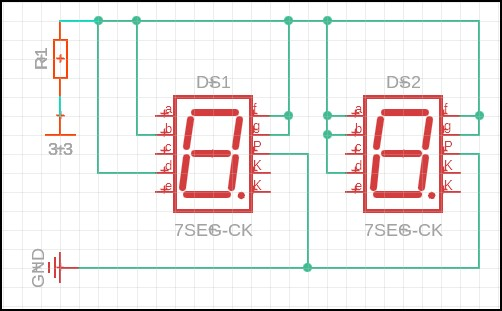
\includegraphics[width=0.6\linewidth]{img/modul_2/schematic_tupen2.jpg}
    \caption{Schematic sesuai nomor kelompok (13)} 
  \end{figure}
\end{enumerate}